\documentclass[conference]{IEEEtran}
\IEEEoverridecommandlockouts
% The preceding line is only needed to identify funding in the first footnote. If that is unneeded, please comment it out.
\usepackage{cite}
\usepackage{amsmath,amssymb,amsfonts}
\usepackage{algorithmic}
\usepackage{graphicx}
\usepackage{textcomp}
\usepackage{xcolor}
\usepackage{listings}
\usepackage{booktabs}
\def\BibTeX{{\rm B\kern-.05em{\sc i\kern-.025em b}\kern-.08em
    T\kern-.1667em\lower.7ex\hbox{E}\kern-.125emX}}
    
\begin{document}

\title{Deep Learning\\
{\footnotesize COS711 Assignment 3 | Student Number: 15024522}
}

\author{\IEEEauthorblockN{Marcus Bornman}
\IEEEauthorblockA{\textit{Department of Computer Science} \\
\textit{University of Pretoria}\\
Pretoria, South Africa \\
u15024522@tuks.co.za}
}

\maketitle

\begin{abstract}
The "Makerere Passion Fruit Disease Detection - presented by The Marconi Society Machine Learning Laboratory at Makerere University - is addressing the classification of passion fruit diseases by developing a low-cost hand-held diagnostic device which makes use of state-of-the-art machine learning techniques. This report details the architecture, experimentation and results of a convolutional neural network inline with this initiative. Results show that more training is needed on the presented neural network, which placed 121st in competition rankings at the time of writing.
\end{abstract}

\begin{IEEEkeywords}
convolutional neural networks, fruit disease Detection
\end{IEEEkeywords}
\section{Introduction}
Convolutional neural networks have become widely known as the state-of-the-art standard in image recognition - a field with numerous practical applications. One of these applications is identified by the "Makerere Passion Fruit Disease Detection Challenge" \cite{zindi}. The challenge - presented by The Marconi Society Machine Learning Laboratory at Makerere University - is addressing the classification of passion fruit diseases by developing a low-cost hand-held diagnostic device which makes use of state-of-the-art machine learning techniques. This report details the architecture, experimentation and results of a convolutional neural network inline with this initiative.

The report is structured such that we first provide the appropriate background on each of the aforementioned concepts, and on the data set. Then, we elaborate on the experimental setup - we detail any data pre-processing that was done, we describe the architecture of the networks, we explain why specific hyper-parameters were chosen for each of the methods, and we note the process utilized to perform experimentation. Penultimately, we present and discuss the results and, finally, we conclude with a summary of the findings and any additional remarks.
\section{Background}
This section will provide details on the problem domain and the algorithms that have been made use of. First, we describe the problem domain in terms of the challenge we are attempting to solve. Then, we provide some background on ResNet50V2 \cite{ResNet50V2} - the network employed for feature extraction in our convectional neural network. Finally, we elaborate on convolutional neural networks, as this is the kind of network we built.

\subsection{Makerere Passion Fruit Disease Detection}\label{sec:domain}
The findings presented in this report are relevant to the "Makerere Passion Fruit Disease Detection Challenge" \cite{zindi}. The challenge entails classifying the disease status of a plant, given an image of a passion fruit.

The images were collected from the various areas in Uganda. Capturing images involved guidance from National Crop Resources Research Institute (NaCRRI) passion fruit disease experts. These experts identified the disease manifestation in the fruits of passion fruit plants.

Roughly, the dataset contains 4000 images. All images have been resized to 512x512 pixels. Some images have more than a single fruit. Thus, some images have more than a single bounding box. Each bounding box is tagged to one of three classes: \emph{fruit\_healthy}, \emph{fruit\_brownspot} and \emph{fruit\_woodiness}.

\subsection{ResNet50V2}
Deep residual networks (ResNets) \cite{resnet} provide a learning framework for deep neural networks in particular. Simply, ResNets "reformulate the layers as learning residual functions with reference to the layer inputs, instead of learning un-referenced functions". ResNets were shown to perform better than state-of-the-art methods of the time. Particularly in the context of networks with considerable depth and with challenging image recognition tasks.

Building on the idea of ResNets, ResNet50V2 \cite{ResNet50V2} was introduced. ResNet50V2 adds a new "residual unit". Results show that ResNet50V2 improved on the performance of ResNet50, both in terms of the ease of training and ability to generalize. In the context of this report, ResNet50 is used for feature extraction in both the identification of bounding boxes and classification of fruits.

\section{Experimental Set-Up} \label{sec:experiment}

This section presents all experimentation details. Starting with what was done for data preparation, then identifying the network architecture and parameters, then explaining experiment runs and how results were captured.

\subsection{Data Preparation}
As mentioned in Section \ref{sec:domain}, the dataset consists of 512x512 images of one or more fruits. In addition, the data set provides labels for the images in the form of a class and the top-left coordinates, height and width of the associated bounding box. In pre-processing the data, we created a data frame wherein the height and width attributes were replaced with the bottom-right coordinates of the bounding box. In addition, we replaced the class labels as follows:
\begin{itemize}
    \item \emph{fruit\_brownspot} would be replaced with 1.
    \item \emph{fruit\_brownspot} would be replaced with 2.
    \item \emph{fruit\_brownspot} would be replaced with 3.
\end{itemize}

Consequently, the following represents a sample of what the data labels looked like at this stage:

\begin{figure}[htbp]
\centerline{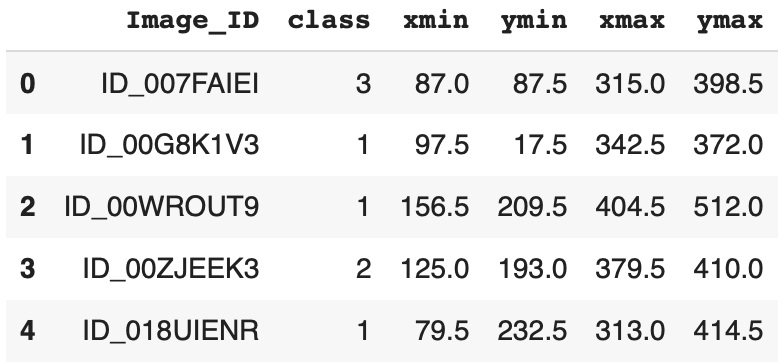
\includegraphics[width=0.5\textwidth]{report/4_experimental/data.png}}
\caption{Image labels after pre-processing.}
\label{fig:data}
\end{figure}

Next, we performed binary one-hot encoding on the classes and scaled the image data itself such that all data was scaled between 0 and 1. This was done because it is required by the Keras \cite{keras} implementation of ResNet50V2 \cite{ResNet50V2}, which we would be using.

Finally, we performed an 80/20 split between the training data and validation data. No split was performed for test data because the competition provided an entirely separate data set for testing purposes.

\subsection{Network Parameters}

For the purposes of this report, we made use of a convolutional neural network architecture which uses ResNet50V2 \cite{ResNet50V2} for the feature extraction segment of the network. In other words, the network comprised a combination of ResNet50V2 \cite{ResNet50V2} - which would not be trained - and 2 branches - one for classifying classes for fruits, and another for identifying bounding boxes.

Each of the 2 branches had one input layer, and single hidden layer and a single output layer. The branch for classifying fruit classes also included 2 dropout layers. For activation functions for the different layers, we made use of ReLU, Sigmoid and Softmax functions. 

For the size of the the first and second layers of each branch - and, for the learning rate - we performed hyperparameter tuning using teh Hyperband Tuner \cite{hyperband}. Following tuning, this was the best hyper-parameter compination that could be found:
\begin{itemize}
    \item \emph{Number of units in the first layer of each branch}: 48
    \item \emph{Number of units in the second layer of each branch}: 32
    \item \emph{Learning rate:} 0.0001
\end{itemize}

\subsection{Running Experiments} \label{sec:experiment_run}
Firstly, note that all experiments were executed using  the Tensorflow framework and the Keras high-level API \cite{keras}. For each of the optimisation and training methods considered, we performed 10 runs. Each run consists of training the network from scratch, for 10 epochs, and testing the networks performance against the test data set.

After 10 test runs had been completed, we calculated the average and standard deviation of the training and validation accuracies across all runs. Additionally, we calculated the average accuracy and sparse categorical crossentropy loss for the test data set across the 10 runs.

All code used to run experiments is available at https://github.com/marcus-bornman/cos\_711\_assignment\_3.
\section{Research Results}
All results reported in this section are based on an average over 10 test runs, as described in Section \ref{sec:experiment_run}. We begin by presenting the performance, in terms of training and validation accuracy, of our approach. We then present a comparison of the average sparse categorical crossentropy loss for our approach and how this progressed during convergence. Finally, we report on the results of submitting our approach to the "Makerere Passion Fruit Disease Detection Challenge" \cite{zindi} and how it compares to other submissions.

\subsection{Accuracy}

Table \ref{tab:results} shows the average training and validation accuracy for classifying the fruits into classes and identifying bounding boxes. In addition, the standard deviation across the 10 runs is also reported.

\begin{table}[htbp]
\caption{Results in terms of accuracy.}
\centerline{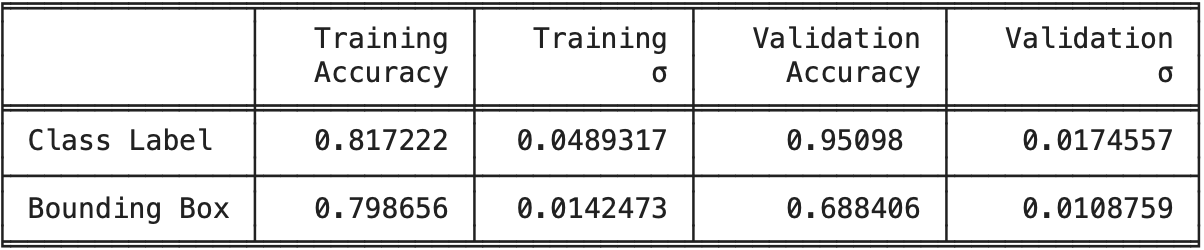
\includegraphics[width=0.5\textwidth]{report/5_results/results.png}}
\label{tab:results}
\end{table}

We note that, in the case of classifying fruit classes, validation accuracies were better than the accuracy achieved for training data. This may be as a result of over-fitting. However, the same is not true for the determination of bounding boxes; and so, we did not make alterations to the learning rate.

\subsection{Loss}
Figure \ref{fig:loss} shows the average sparse categorical crossentropy loss on the training and validation sets, for each approach.

\begin{figure}[htbp]
\centerline{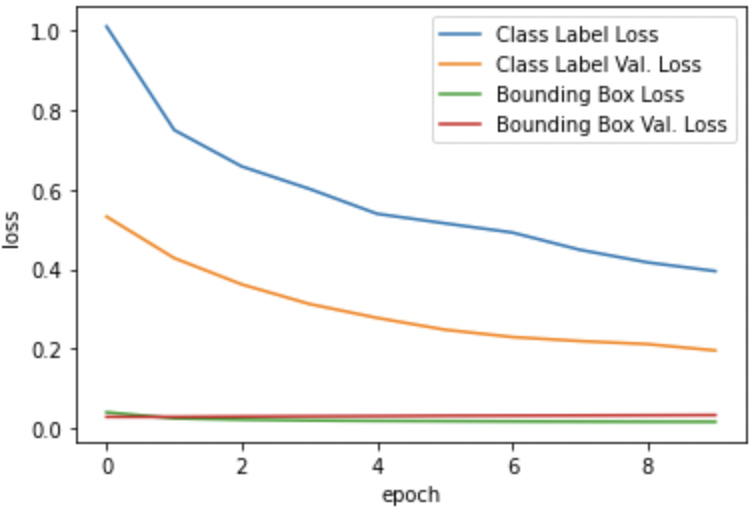
\includegraphics[width=0.4\textwidth]{report/5_results/loss.png}}
\caption{Progression of loss during training.}
\label{fig:loss}
\end{figure}

As can be seen, the loss for both the training and validation sets in the context of identifying bounding boxes was minimal from the start of training. This is due the the efficacy of ResNet50V2 \cite{ResNet50V2}, which had already been trained prior to the training of our model.

In addition, we can see that - in the context of classifying fruits, the network had not yet fully converged. This is likely because we had only trained the network for 10 epochs. It is also notable that the network seemed to generalse well in that validation loss was consistently lower than training loss for the classification of fruits.

\subsection{Comparison}
Upon submission to the "Makerere Passion Fruit Disease Detection Challenge" \cite{zindi}, our network received a score of around 0.30696. At the time of writing, this ranked it 121st on the leaderboard for the competition. It was also quite a ways of the leaders who had scored 0.90311.
\section{Conclusion(s)}
This report presented the results of using a Convolutional Neural Network - partly comprising ResNet50V2 \cite{ResNet50V2} - to identify bounding boxes and classify fruits as per the competition detailed by the "Makerere Passion Fruit Disease Detection Challenge" \cite{zindi}.

Using a simple network architecture that extends ResNet50V2 \cite{ResNet50V2} with 2 branches, the results show promise, but further research is needed with additional training emphasised as one of the shortfalls of existing experimentation. The model presented was submitted to Zindi \cite{zindi} and placed 121st in the rankings for the competition at the time of writing.
\begin{thebibliography}{00}
\bibitem{zindi} “Makerere Passion Fruit Disease Detection Challenge.” Zindi, The Marconi Society Machine Learning Laboratory, zindi.africa/competitions/makerere-passion-fruit-disease-detection-challenge.
\bibitem{resnet} He, Kaiming, et al. "Deep residual learning for image recognition." Proceedings of the IEEE conference on computer vision and pattern recognition. 2016.
\bibitem{ResNet50V2} He, Kaiming, et al. "Identity mappings in deep residual networks." European conference on computer vision. Springer, Cham, 2016.
\bibitem{hyperband} Li, Lisha, et al. "Hyperband: A novel bandit-based approach to hyperparameter optimization." The Journal of Machine Learning Research 18.1 (2017): 6765-6816.
\end{thebibliography}

\end{document}